\section{Content}
\label{section:content}

\subsection{DDoS Attacks and BRO}\label{subsec:ddos-and-bro}
In this section we will first define the notion of a DDoS attack by explaining how the infrastructure looks like. Then we will elaborate on various DDoS attacks used nowadays and discuss their main characteristics. After this we will discuss the syntax of the detection rules of the BRO SIDS.

\subsubsection{The DDoS Attack}
Figure \ref{fig:ddos-overview} shows the infrastructure of a DDoS attack. Actors involved in a DDoS attack are denoted by a letter (A-D) whereas data streams are denoted by numbers (1-5). 

A DDoS attack starts with an attacker (A). The attacker sends data needed to start the attack (1) to the Command and Control (C\&C) servers (B). The C\&C servers control the infected machines (C). The infected machines are also known under the name of bots. The C\&C servers plus the infected machines are more commonly named as a botnet. The C\&C servers send a message (2) to the infected machines. In case of the Ramnit botnet, only the infected machines counted 3.2 million machines \cite{europol2015}. At this point two paths are used to get to the target machine (E). The first path possible is aiming the infected machines directly to the target (4). The second path possible is using public services (D) like a DNS to reach the target (5). 

In the next subsection we will describe various types of DDoS attacks. 

\begin{figure}[H]
\centering
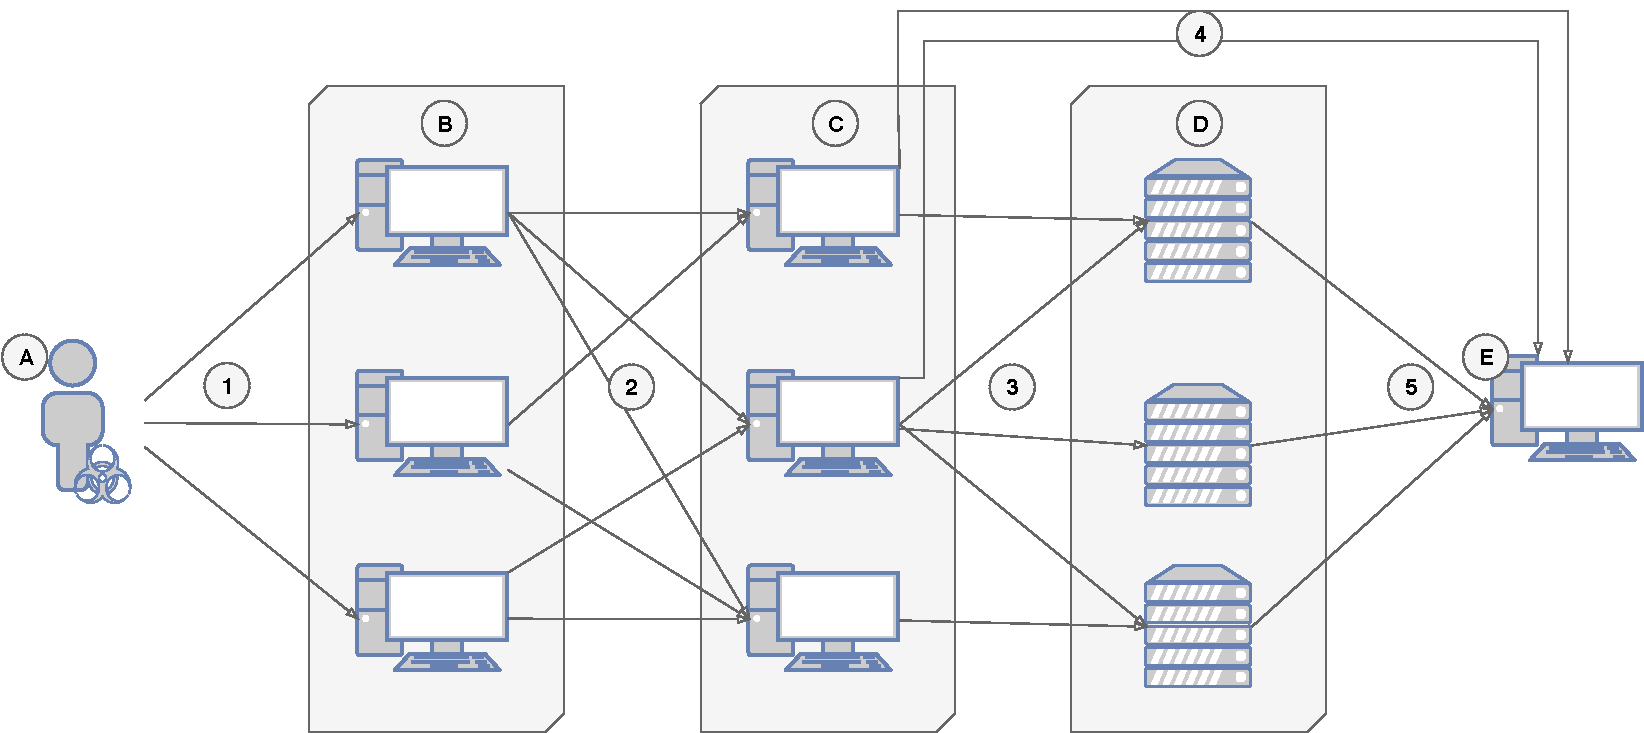
\includegraphics[width=\textwidth]{./images/ddos-overview.pdf}
\caption{Overview of DDoS attack infrastructure}
\end{figure}\label{fig:ddos-overview}

\subsubsection{Types of Attacks}
In this section we will briefly elaborate on the most common types of attack mentioned in the security report of Akami Q4 2017 \cite{Akamai2017-4}. An overview of the main characteristics per attack can be found in Table \ref{tab:attack-overview}.


\paragraph{UDP}
The UDP attack exploits UDP. The attack consists of sending a large number of packets to random ports of the target. Hereby the target machine will check if an application listens to this port and if not will reply with an ICMP Destination Unreachable packet. Looking at Figure \ref{fig:ddos-overview}, path 4 is used.

\paragraph{UDP Fragment}
The UDP Fragmantation attack exploits the fragmentation used in the IP protocol \cite{imperva}. When a packet is to big to be sent across a network link, it will be broken down into smaller packets and later on resembled again. In a UDP Fragmentation attack, fraudulent UDP packets are sent which are larger than the maximum transmission unit (MTU) of the network. The idea is that the packets can not be reassembled and thereby consuming the server's resources. 

\paragraph{DNS}
The DNS attack exploits the public Domain Name System (DNS) services on the internet. DNS is used to resolve IP adresses from website names. In a DNS attack the attacker spoofs its IP replacing its IP with that of the target. The DNS server sees the request as it came from the target and replies as if it were a normal request. This way of attacking allows an attacker to amplify its own bandwidth by using the asymmetry between request and response size. Looking at Figure \ref{fig:ddos-overview}, path 5 is used. The attack runs over UDP.  

\paragraph{NTP}
The NTP attack exploits the public Network Time Protocol (NTP) services on the internet. NTP services allow for time synchronization between machines. This attack is similar to the DNS attack, but this time the NTP services instead of the DNS services are used. 

\paragraph{Chargen}
The Chargen attack exploits the public Character Generator Protocol (Chargen). Once a Chargen services receives a packet via UDP, it responds by sending a datagram containing a random number between 0 and 512 characters long \cite{ietf1983}. The attack approach works the same as the NTP and DNS attacks.  

\paragraph{CLDAP}
The CLDAP attack exploits the Connection-less Lightweight Directory Access Protocol (CLDAP). CLDAP is designed to provide access to directories while not needing the recourse requirements of the Directory Access Protocol (DAP) \cite{ietf1995}. The attack is similar to the DNS, NTP and Chargen attack. 

\paragraph{SYN}
The SYN attack exploits the three-way handshake of TCP. During this attack a large number of SYN packets are send to the target machine. The target machine will respond by sending a SYN-ACK packet. The attacker at this point does not respond by sending an ACK packet, leaving the connection half initialized. This way the attacker keeps connections from being used by legitimate users. Compared to the attacks mentioned above, this one runs over TCP rather than UDP. In this attack, path 4 is used. 

\paragraph{SSDP}
The SSDP attack exploits the Simple Service Discovery Protocol (SSDP). SSDP is used to discover network services. The attack is similiar to DNS, NTP and Chargen but when looking to Figure \ref{fig:ddos-overview} the machines in D are for instance home routers, printers or other IOT devices rather than a dedicated server. 


\paragraph{ACK}
The ACK attack exploits TCP. During this attack a large number of ACK packets are send towards the target. These ACKs do not belong to any connection and are therefore dropped at the target machine. This however does deplete resources of the target. The attack runs via path 4.  


\paragraph{RPC}
?

\paragraph{HTTP}
Rather than the attacks mentions above, the HTTP attack targets the application layer. The attack consists of sending a large number of HTTP requests (like GET, PUSH and POST) to the target, hereby depleting its resources. Looking at Figure \ref{fig:ddos-overview}, path 4 is used.



\begin{table}
\centering
\begin{tabular}{l | l}
Attack Type & Main Characteristics \\ \hline \hline
UDP Frag & IPv4 \&\& fragments \\ \hline
DNS & UDP \&\& src\_port==53 \&\& DNS\_query \&\& DNS\_type \\ \hline
CLDAP & UDP \&\& src\_port==389 \\ \hline
NTP & UDP \&\& src\_port==123 \\ \hline
UDP & UDP \\ \hline
Chargen & UDP \&\& src\_port==19 \\ \hline
SYN & TCP \&\& flag==SYN \\ \hline
SSDP & UDP \&\& src\_port==1900 \\ \hline
ACK & TCP \&\& flag==ACK \\ \hline
RPC & ? \\ \hline
HTTP & HTTP \&\& HTTP\_request \&\& src\_port==80
\end{tabular}
\caption{\label{tab:attack-overview}Attack types main characteristic overview.}
\end{table}


\subsubsection{BRO Rule Syntax} 


\subsection{Methodology}\label{subsec:methodology}

\subsection{Evaluation and Discussion}\label{subsec:evaluation-discussion}
\subsubsection{Evaluation}\label{subsubsec:evalutation}
\subsubsection{Discussion}\label{subsubsec:discussion}
